\documentclass[12pt]{jsarticle}
\pagenumbering{arabic}
\usepackage{listings,jlisting}
\usepackage{url}
\usepackage[dvipdfmx]{graphicx}
\usepackage{amsmath}
\usepackage{ascmac}
\usepackage{cases}

\lstset{
  language=,
  basicstyle={\small},%
  identifierstyle={\small},%
  commentstyle={\small\itshape\color[rgb]{0,0.5,0}},%
  keywordstyle={\small\bfseries\color[rgb]{0,0,1}},%
  ndkeywordstyle={\small},%
  stringstyle={\small\ttfamily\color[rgb]{1,0,1}},
  frame={tb},
  breaklines=true,
  columns=[l]{fullflexible},%
  numbers=left,%
  xrightmargin=0zw,%
  xleftmargin=3zw,%
  numberstyle={\scriptsize},%
  stepnumber=1,
  numbersep=1zw,%
  lineskip=-0.5ex%
}

\begin{document}

今回の課題では図\ref{fig:kairo}の回路に流れる電流の値をガウスの消去法、ヤコビ法、ガウスザイデル法を用いて求めることを目的とする。
\begin{figure}[h]
	\centering
	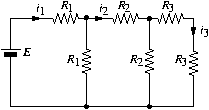
\includegraphics[clip,width=5.0cm]{./kairo.png}
	\caption{電流の値が不明な回路図}
	\label{fig:kairo}
\end{figure}

$E = 20[V], R_1 = 20[\Omega], R_2= 10[\Omega], R_3 = 17[\Omega] となっている。これらをもとにしてi_1, i_2, i_3 を求める。$

これらから連立方程式を立てると
\begin{eqnarray}
	\begin{cases}
		2R_1i_1 - R_1i_2 = E & \\
		R_1i_1 + 2R_2i_2 - R_2i_3 = E & \\
		R_1i_1 + R_2i_2 + 2R_3i_3 = E
	\end{cases}
\end{eqnarray}

$i$について整理すると
\begin{eqnarray}
	\begin{cases}
		i_1 = \frac{E + R_1i_2}{2R_1} &\\
		i_2 = \frac{E -R_1i_1 + R_2i_3}{2R_2} &\\
		i_3 = \frac{E -R_1i_1 - R_2i_2}{2R_2}
	\end{cases}
\end{eqnarray}

これらの式を用いて$i$について求める。

なお手動でもとめると以下のようになる。

\begin{numcases}
	{}
	i_1 = E / (R_1 + \frac{1}{ \frac{1}{R_1} + \frac{1}{ R_2 + \frac{1}{ \frac{1}{2R_3} + \frac{1}{R_2}}}}) & \\
	i_2 = 2i_1 - \frac{E}{R_1} & \\ 
	i_3 = 2i_2 + \frac{i_1R_1}{R_2} - \frac{E}{R_2}  &
\end{numcases}

計算すると $i_1 = 0.680327868852459, i_2 = 0.360655737704918, i_3 = 0.0819672131147541$という結果になった。なお、実際に値を求める際には上の式をプログラムに入力した。

\section{課題1}
\subsection{ヤコビ法を基にしたガウスザイデル法の作製}
まずヤコビ法を実装したプログラム(\cite{yacobiurl}から引用)をソースコード\ref{lst:yacobi}に示す。

\begin{lstlisting}[caption=yacobi.c,label={lst:yacobi}]
/*
  Yacobi  method
*/

#include <stdio.h>
#include <math.h>
#define n 4
#define n1 5
#define EPS 1.0e-15
#define KMAX 100

main()
{
	int i,j,k=0,l;
	double a[n1][n1],b[n1],x[n1],xn[n1],eps_sum;
	
		a[1][1]=4;  a[1][2]=1;  a[1][3]=0;  a[1][4]=-2;
		a[2][1]=1;  a[2][2]=4;  a[2][3]=-1; a[2][4]=1;
		a[3][1]=0;  a[3][2]=-1; a[3][3]=4;  a[3][4]=-1;
		a[4][1]=-2; a[4][2]=1;  a[4][3]=-1; a[4][4]=4;
		b[1]=5,     b[2]=-5,    b[3]=6,     b[4]=8;
		x[1]=0,     x[2]=0,     x[3]=0,     x[4]=0;
	
	do{
		eps_sum=0.0;
		for(i=1; i<=n; i++){
			xn[i]=b[i];
			for(j=1; j<=n; j++){
				if(j!=i) xn[i] -= a[i][j]*x[j];
			}
			xn[i] /=a[i][i];
		}
		for(i=1; i<=n; i++){
			eps_sum +=fabs(xn[i]-x[i]);
			x[i]=xn[i];
		}
		k++;
	}while(eps_sum>EPS && k< KMAX);
	if(k == KMAX){
		printf("Error!! The answers is not found.\n");
	}else{
		printf(" Iteration K = %d \n",k);
		for(i=1; i<=n; i++){
			printf( "x[%d] = %f ",i,x[i]);
		}
		printf(" \n");
	}
}
\end{lstlisting}
\subsection{ガウスザイデル法の作製}
ソースコード\ref{lst:yacobi}を基にして、ガウスザイデル法のプログラムを作製する。ヤコビ法とガウスザイデル法との大きな違いとして、ガウスザイデル法では今現在わかっている最新の変数の値を基に変数を求めることが挙げられる。ソースコード\ref{lst:gauss_seidel}にガウスザイデル法を示す。
\begin{lstlisting}[caption=gauss\_seidel.c,label={lst:gauss_seidel}]
/*
  Gauss-seidel method
*/

#include <stdio.h>
#include <math.h>
#define n 4
#define n1 5
#define EPS 1.0e-15
#define KMAX 100

main()
{
	int i,j,k=0,l;
	double a[n1][n1],b[n1],x[n1],xn[n1],eps_sum;
	
		a[1][1]=4;  a[1][2]=1;  a[1][3]=0;  a[1][4]=-2;
		a[2][1]=1;  a[2][2]=4;  a[2][3]=-1; a[2][4]=1;
		a[3][1]=0;  a[3][2]=-1; a[3][3]=4;  a[3][4]=-1;
		a[4][1]=-2; a[4][2]=1;  a[4][3]=-1; a[4][4]=4;
		b[1]=5,     b[2]=-5,    b[3]=6,     b[4]=8;
		x[1]=0,     x[2]=0,     x[3]=0,     x[4]=0;
	
	do{
		eps_sum=0.0;
		for(i=1; i<=n; i++){
			ox = x[i];
			x[i]=b[i];
			for(j=1; j<=n; j++){
				if(j!=i) x[i] -= a[i][j]*x[j];
			}
			x[i] /= a[i][i];
			eps_sum +=fabs(x[i]-ox);
		}
		k++;
	}while(eps_sum>EPS && k< KMAX);
	if(k == KMAX){
		printf("Error!! The answers is not found.\n");
	}else{
		printf(" Iteration K = %d \n",k);
		for(i=1; i<=n; i++){
			printf( "x[%d] = %f ",i,x[i]);
		}
		printf(" \n");
	}
}
\end{lstlisting}
配列xを常に現在わかっている最新のものが入れられるようになる。
\section{課題2}
では実際にプログラムを使用し、iについて求めていく。
\subsection{課題2の結果}
結果を以下に示す。
Kはプログラムの反復回数を表し、timeは値を求めた開始から終了までの秒数を示している。

\begin{screen}
\$ ./a.out \\
Yacobi \\
 Iteration K = 193 \\
x[1] = 0.680328 x[2] = 0.360656 x[3] = 0.081967 \\
time: 0.000011 \\
\\
Gauss\_seidel \\
 Iteration K = 37 \\
x[1] = 0.680328 x[2] = 0.360656 x[3] = 0.081967 \\
time: 0.000002 \\
\\
Gaussian \\
x[1] = 0.680328 x[2] = 0.360656 x[3] = 0.081967 \\
time: 0.000001
\end{screen}

\subsection{考察}
実行結果を見るとどの結果も手動で求めたものと同じものであることから、プログラムはすべて正しいことがわかる。しかし、反復回数、実行速度を見てみると、それぞれに違いがある。この中で最も最速で求めることができるのはガウスの消去法である。しかし、このあとのソースコード\ref{lst:answer}を確認してもらいたいのだが、コード量が他の2つよりも多くなる。それに比べ、ガウスザイデル法はヤコビ法と大きく変わらない。これだけのコードの変更で5倍の速さで求められることは効率が良いといえる。必要とするものによってかわるが、スピードが重要でないのであれば、実装のしやすさ等を考慮し、ガウスザイデル法を選ぶ、といったことも考えられる。


\subsection{使用したプログラム}

ソースコード\ref{lst:answer}にガウスの消去法、ヤコビ法、ガウスザイデル法を用いて求めた結果を出力するプログラムを示す。なお、このプログラムは上記のソースコード\ref{lst:yacobi}、\ref{lst:gauss_seidel}及び\cite{gaussian}のプログラムを引用、改変したものである。

\begin{lstlisting}[caption=answer.c,label={lst:answer}]
#include <stdio.h>
#include <math.h>
#include <sys/time.h>

#define n 3
#define n1 4
#define EPS 1.0e-15
#define KMAX 10000

void yacobi()
{
	struct timeval t0;
	struct timeval t1;
	int i,j,k=0,l;
	int count;
	double a[n1][n1],b[n1],x[n1],xn[n1],eps_sum;
	printf("Yacobi\n");
	
		a[1][1]=2*20;	a[1][2]=-20;	a[1][3]=0;
		a[2][1]=20;		a[2][2]=2*10;	a[2][3]=-10;
		a[3][1]=20;		a[3][2]=10;		a[3][3]=2*17;
		b[1]=20,		b[2]=20,		b[3]=20;
		x[1]=0,			x[2]=0,			x[3]=0;
	
	gettimeofday(&t0, NULL);
	do{
		eps_sum=0.0;
		for(i=1; i<=n; i++){
			xn[i]=b[i];
			for(j=1; j<=n; j++){
				if(j!=i) xn[i] -= a[i][j]*x[j];
			}
			xn[i] /=a[i][i];
		}

		for(i=1; i<=n; i++){
			eps_sum +=fabs(xn[i]-x[i]);
			x[i]=xn[i];
		}
		k++;
	}while(eps_sum>EPS && k< KMAX);
	gettimeofday(&t1, NULL);
	if(k == KMAX){
		printf("Error!! The answers is not found.\n");
	}else{
		printf(" Iteration K = %d \n",k);
		for(i=1; i<=n; i++){
			printf( "x[%d] = %f ",i,x[i]);
		}
		printf(" \n");
		printf("time: ");
		printf("%d.%06d\n", t1.tv_sec - t0.tv_sec, t1.tv_usec - t0.tv_usec);
		printf(" \n");
	}
}

void gauss_seidel()
{
	struct timeval t0;
	struct timeval t1;
	int i,j,k=0,l;
	double a[n1][n1],b[n1],x[n1],xn[n1],ox,eps_sum;
	printf("Gauss_seidel\n");
	
		a[1][1]=2*20;	a[1][2]=-20;	a[1][3]=0;
		a[2][1]=20;		a[2][2]=2*10;	a[2][3]=-10;
		a[3][1]=20;		a[3][2]=10;		a[3][3]=2*17;
		b[1]=20,		b[2]=20,		b[3]=20;
		x[1]=0,			x[2]=0,			x[3]=0;
	
	gettimeofday(&t0, NULL);
	do{
		eps_sum=0.0;
		for(i=1; i<=n; i++){
			ox = x[i];
			x[i]=b[i];
			for(j=1; j<=n; j++){
				if(j!=i) x[i] -= a[i][j]*x[j];
			}
			x[i] /= a[i][i];
			eps_sum +=fabs(x[i]-ox);
		}
		k++;
	}while(eps_sum>EPS && k< KMAX);
	gettimeofday(&t1, NULL);
	if(k == KMAX){
		printf("Error!! The answers is not found.\n");
	}else{
		printf(" Iteration K = %d \n",k);
		for(i=1; i<=n; i++){
			printf( "x[%d] = %f ",i,x[i]);
		}
		printf(" \n");
		printf("time: ");
		printf("%d.%06d\n", t1.tv_sec - t0.tv_sec, t1.tv_usec - t0.tv_usec);
		printf(" \n");
	}
}

void gaussian()
{
	struct timeval t0;
	struct timeval t1;
	int i,j,k,ip;
	double a[n1][n1],b[n1],x[n1],w,m,s,amax,tmp;
	printf("Gaussian\n");
	
		a[1][1]=2*20;	a[1][2]=-20;	a[1][3]=0;
		a[2][1]=20;		a[2][2]=2*10;	a[2][3]=-10;
		a[3][1]=20;		a[3][2]=10;		a[3][3]=2*17;
		b[1]=20,		b[2]=20,		b[3]=20;

	
	gettimeofday(&t0, NULL);
	for(k=1 ; k<=n-1; k++){
		/* pivot selection */
		amax=fabs(a[k][k]);
		ip=k;
		for(i=k+1;i<=n;i++){
			if( fabs(a[i][k])> amax){
				amax=fabs(a[i][k]);
				ip=i;
			}
		}
	  
		if(ip != k){
			for(j=k; j<=n; j++){
				tmp=a[k][j];
				a[k][j]=a[ip][j];
				a[ip][j]=tmp;
			}
			tmp=b[k];
			b[k]=b[ip];
			b[ip]=tmp;
		}

		/* Forward */
		w=1.0/a[k][k];
		for(i=k+1; i<=n; i++){
			m=a[i][k]*w;
			for(j=k+1; j<=n; j++){
				a[i][j]-=m*a[k][j];
			}
			b[i]-=m*b[k];
		}
	}
	
	/* Backward */
	x[n]=b[n]/a[n][n];
	for(k=n-1; k>=1; k--){
		s=0;
		for(j=k+1; j<=n; j++){
			s+=a[k][j]*x[j];
		}
		x[k]=(b[k]-s)/a[k][k];
	}
	gettimeofday(&t1, NULL);
	for(i=1; i<=n; i++){
		printf("x[%d] = %f ",i,x[i]);
	}
	printf(" \n");
	printf("time: ");
	printf("%d.%06d\n", t1.tv_sec - t0.tv_sec, t1.tv_usec - t0.tv_usec);
}

int main(void) {
	yacobi();	
	gauss_seidel();
	gaussian();
}
\end{lstlisting}



\begin{thebibliography}{9}
	\bibitem{yacobiurl} 片山英昭 ヤコビ法ソースコード \url{http://moodle.maizuru-ct.ac.jp/moodle/file.php/184/yacobi.c}
	\bibitem{gaussian} 片山英昭 ガウスの消去法ソースコード \url{http://moodle.maizuru-ct.ac.jp/moodle/file.php/184/gauss_pivot.c}
\end{thebibliography}
\end{document}

